\documentclass[../main.tex]{subfiles}
 
\begin{document}

\chapter{Variational Monte Carlo}

The Variational Monte Carlo method the main computational method used in this thesis. It is based on the variational principle in quantum mechanics. The variational principle states that, given a Hamiltonian $H$ and a trial wave function $\psi_T$, the expectation value $\langle H \rangle$ defined as\cite{Griffiths}
\begin{equation}
 E[H] = \langle H \rangle =
 \frac{\int d {\bf R} \Psi_T^*({\bf R}, \boldsymbol{\alpha}) H({\bf R}) \Psi_T({\bf R}, \boldsymbol{\alpha})}
       {\int d {\bf R} \Psi_T^*({\bf R}, \boldsymbol{\alpha}) \Psi_T({\bf R}, \boldsymbol{\alpha})}
 \label{multidim}
\end{equation}
is an upper bound to the ground state energy $E_0$ of the Hamiltonian, i.e.
\begin{equation}
E_0 \leq \langle H \rangle.
\end{equation}
Here our trial wave function is dependant on some variational parameters $\boldsymbol{\alpha}$, and the goal of the VMC method is to vary these parameters until we find the lowest possible value of $\langle H\rangle$ in order to get an estimate for the ground state energy $E_0$. In general, the integrals we have to compute to find $\langle H\rangle$ are multi-dimensional ones, so using traditional integration methods like Gauss-Legendre is too computationally expensive. Therefore we turn to Monte Carlo methods.

\section{Metropolis Sampling}

\subsection{Monte Carlo Integration with Brute Force Metropolis Sampling}
This description of Monte Carlo integration and the Metropolis algorithm follows Ref.~\cite{FYS4411-Slides}.
For a given trial wave function we define a probability distribution function (PDF)
\begin{equation}
 P({\bf R}) = \frac{|\Psi_T({\bf R})|^2}{\int |\Psi_T({\bf R})|^2 d{\bf R}}
\end{equation}
Together with the local energy given in Eq.(\ref{eq: E_L}) we have that the approximation to the expectation value of the Hamiltonian is
\begin{align}
\begin{split}
E[H(\mathbf{\alpha})] =& \int P({\bf R}) E_L({\bf R}) d{\bf R}\\
\approx& \frac{1}{N} \sum_{i=1}^N P({\bf R}_i, \boldsymbol{\alpha}) E_L({\bf R}_i, \boldsymbol{\alpha}),
\end{split}
\end{align}
where $N$ is the number of Monte Carlo samples, $\mathbf{R_i}$ are the positions of the particles at step $i$ and $\boldsymbol{\alpha}$ are the variational parameters.

The Metropolis algorithm is used to sample the probability distribution by a stochastic process. We define ${\bf P}_i^{(n)}$ to be the probability for finding the system in the state $i$ at step $n$, and the algorithm is then
\begin{itemize}
 \item Sample a possible new state $j$ with some probability $T_{i\rightarrow j}$
 \item Accept the new state with probability $A_{i\rightarrow j}$ and use it as the next sample, or with probability $1 - A_{i\rightarrow j}$, reject the move and use the original state $i$ as sample again.
\end{itemize}
We want to ensure that ${\bf P}_i^{(n\rightarrow \infty)} \rightarrow p_i$, so that regardless of the initial distribution, the method converges to the correct distribution. To ensure this we demand that the transition probability $T$ and the acceptance probability $A$, fulfill the detailed balance requirement
\begin{equation}\label{eq: DB}
 \frac{A_{i\rightarrow j}}{A_{j\rightarrow i}} = \frac{p_i T_{i\rightarrow j}}{p_j T_{j\rightarrow i}},
\end{equation}
where $p_i = P({\bf R}_i)$ and $p_j = P({\bf R}_j)$.
The Metropolis algorithm then uses the following ratio of probabilities to determine whether or not to accept a move
\begin{equation}\label{eq: ratio}
 \frac{p_j}{p_i} = \frac{T_{i\rightarrow j} A_{i\rightarrow j}}{T_{j\rightarrow i} A_{j\rightarrow i}}
\end{equation}
When using the Metropolis algorithm we can either use brute force or importance sampling. If we use the brute force Metropolis algorithm, we assume that $T_{i\rightarrow j} = T_{j\rightarrow i}$. Then the ratio used by the Metropolis algorithm is only dependant on the acceptance probabilities, i.e. the ratio is given by
\begin{equation}\label{ratio2}
 w = \frac{p_j}{p_i} = \frac{A_{i\rightarrow j}}{ A_{j\rightarrow i}} = \frac{|\Psi_T({\bf R}_j)|^2}{|\Psi_T({\bf R}_i)|^2}
\end{equation}
The algorithm for estimating the ground state energy given a set of variational parameters $\mathbf{\alpha}$ is then
\begin{itemize}
 \item Fix the number of Monte Carlo steps and create an initial state            $\bf{R}$ using the given variational parameters
       $\boldsymbol{\alpha}$. Set a step size $\Delta {\bf R}$ and calculate $|\Psi_T^\alpha(\bf{R})|^2$.
 \item Initialize the local energy and start the Monte Carlo calculations.
 \begin{itemize}
     \item Choose a random particle and update its position in order to create a trial state: ${\bf R}_p = {\bf R} + r\Delta {\bf R}$ where $r$ is a random variable $r \in [0,1]$
     \item Calculate $|\Psi_T^\alpha(\bf{R}_p)|^2$ and use the Metropolis algorithm to accept or reject the move by calculating the ratio $w$. 
       If $w \geq s$, where $s$ is a random number $s \in [0,1]$, the new state is accepted. Otherwise we keep the old state.
     \item If the new state is accepted, then we set ${\bf R} = {\bf R}_p$.
     \item Update the local energy.
 \end{itemize}
 
 \item Finish and compute the final estimate for the ground state energy.
\end{itemize}

\begin{figure}[!ht]
    \centering
    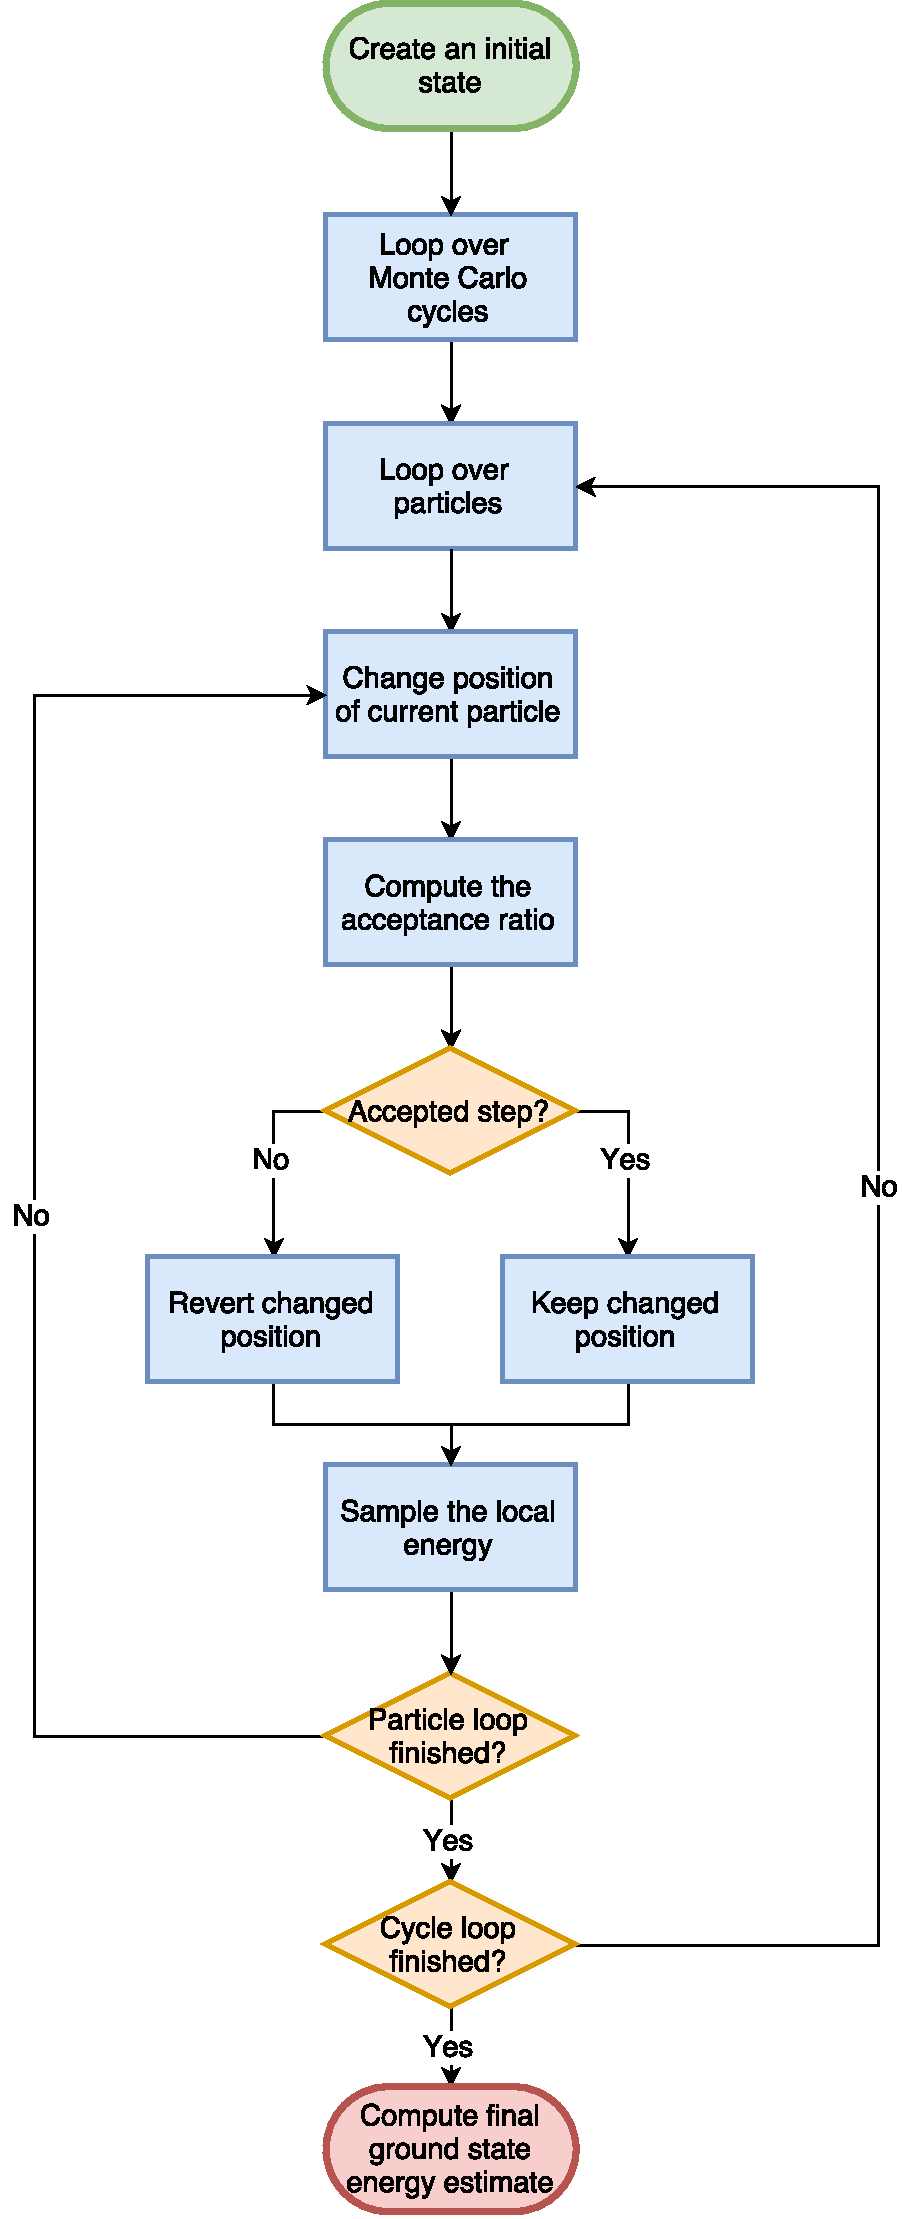
\includegraphics[scale=0.5]{figures/Metropolis_Flowchart}
    \caption{Flowchart of the Metropolis algorithm used in a variational Monte Carlo simulation. The variational parameters, number of Monte Carlo cycles, and various parameters (e.g. number of particles) are set before creating the initial state. The position change and acceptance ratio we use depend on whether we use the regular Metropolis algorithm (brute force), or the Metropolis-Hastings algorithm (importance sampling).}
    \label{fig: Metropolis_Flowchart}
\end{figure}

\subsection{Metropolis-Hastings Algorithm (Importance Sampling)}

For the description of the Metropolis-Hastings Algorithm we again follow Ref.~\cite{FYS4411-Slides}.
When using importance sampling the walk in coordinate space is biased by the trial wave function, so the walker is more likely to move towards regions where the trial wave function is large. The trajectory in coordinate space is generated by the Fokker-Planck equation and the Langevin equation. To find the new positions in coordinate space we solve the Langevin equation using Euler's method. The Langevin equation
\begin{equation}\label{Langevin}
 \frac{\partial x(t)}{\partial t} = D F(x(t)) + \eta,
\end{equation}
where $\eta$ is a random variable and $D$ is the diffusion coefficient, gives the new position
\begin{equation}\label{eq: LangevinSolution}
 y = x + DF(x)\Delta t + \xi \sqrt{\Delta t},
\end{equation}
where $\xi$ is gaussian random variable, $\Delta t$ is a chosen time step and $F(x)$ is the function responsible for drifting the walker towards regions where the wave function is large. $\Delta t$ is treated as a parameter and $\Delta t \in [0.001, 0.01]$ generally yields fairly stable values of the ground state energy. The diffusion coefficient $D$ is equal to $1/2$ and comes from the $1/2$ factor in the kinetic energy operator. The Fokker-Planck equation describes the process of isotropic diffusion characterized by a time-dependent probability density $P(x, t)$ and is given by
\begin{equation}
 \frac{\partial P}{\partial t} = \sum_i D \frac{\partial}{\partial {\bf x}_i}\left( \frac{\partial}{\partial {\bf x}_i} - {\bf F}_i \right) P({\bf x}, t),
\end{equation}
where $\bf{F}_i$ is the $i^{th}$ component of the drift term. By setting the left hand side to zero we obtain the convergence to a stationary probability density. For the resulting equation to be satisfied all the terms of the sum have to be equal to zero, i.e.
\begin{equation}\label{stationaryFokker}
 \frac{\partial^2 P}{\partial {\bf x}_i^2} = P \frac{\partial}{\partial {\bf x}_i} {\bf F}_i
 + {\bf F}_i \frac{\partial}{\partial {\bf x}_i} P.
\end{equation}
The drift vector $\bf{F}$ should be on the form ${\bf F} = g({\bf x}) \frac{\partial P}{\partial {\bf x}}$, which gives us
\begin{equation}\label{stationaryFokkerF}
 \frac{\partial^2 P}{\partial {\bf x}_i^2} = P \frac{\partial g}{\partial P} \left(\frac{\partial P}{\partial {\bf x}_i}\right)^2 + Pg\frac{\partial^2 P}{\partial {\bf x}_i^2}
 + g\left(\frac{\partial P}{\partial {\bf x}_i}\right)^2.
\end{equation}
The condition of stationary density requires that the terms cancel each other out, and that is only possible if $g = \frac{1}{P}$. This leads to
\begin{equation}
 {\bf F} = 2 \frac{1}{\Psi_T} \nabla \Psi_T,
\end{equation}
which is the so-called \textit{quantum force}. By pushing the walker towards regions where the trial wave function is large, this term increases the efficiency of the simulation compared to the brute force Metropolis algorithm where the walker has the same probability of moving in every direction.

From the Fokker-Planck equation we get a transition probability given by the Green's function
\begin{equation}
    G(y, x, \Delta t) = \frac{1}{(4\pi D\Delta t)^{3N/2}}\exp(-(y - x - D\Delta tF(x))^2/4D\Delta t),
\end{equation}
which means that the ratio used in the Metropolis algorithm
\begin{equation}\label{ratio3}
 w = \frac{|\Psi_T({\bf R}_j)|^2}{|\Psi_T({\bf R}_i)|^2} = q(y, x) = \frac{|\Psi_T(y)|^2}{|\Psi_T(x)|^2},
\end{equation}
is now replaced by
\begin{equation}\label{ratio4}
    q(y, x) = \frac{G(x, y, \Delta t)|\Psi_T(y)|^2}{G(y, x, \Delta t)|\Psi_T(x)|^2}.
\end{equation}
Using this ratio and Eq.(\ref{eq: LangevinSolution}), the algorithm is called the Metropolis-Hastings algorithm.


\subsection{Metropolis Sampling with a Slater Determinant}

When our trial wave function contains a Slater determinant we can manipulate it to improve the performance of the code by avoiding calculating the entire determinant at every Metropolis step. The ratio used in Metropolis sampling is given by (Ref.~\cite{FYS4411-Slides})
\begin{align}
    R = \frac{|\hat{D}({\bf r}^{\textrm{new}})|}{|\hat{D}({\bf r}^{\textrm{old}})|} \frac{\Psi_C^{\textrm{new}}}{\Psi_C^{\textrm{old}}},
\end{align}
where $|\hat{D}|$ is the Slater determinant and $\Psi_C$ is the correlation part of the wave function, while "new"and "old" refer to the position before and after a proposed move. If we move only one electron at the time, only a single row in the Slater determinant changes. By doing the calculations in section \ref{sec:ClosedFormMany}(Appendix A.2), we can calculate the Slater determinant part of $R$ using the following formula
\begin{align}\label{eq:MetropolisRatioSD}
    R_{SD} = \sum_{j=1}^N \phi_j({\bf r}_i^{\textrm{new}}) d_{ji}^{-1}({\bf r}^{\textrm{old}}),
\end{align}
where $\phi_j({\bf r}_i^{\textrm{new}})$ are the single particle wave functions evaluated at the new position, and $d_{ji}^{-1}({\bf r}^{\textrm{old}})$ are the elements on the $i$-th column of the inverse Slater matrix $\hat{D}^{-1}$. In addition we need to maintain the inverse matrix by using an updating algorithm whenever a move is accepted. This updating algorithm is also covered in section \ref{sec:ClosedFormMany}, and the equations used are 
\begin{align}
    d^{-1}_{kj}(\mathbf{r}^{\textrm{new}}) = \left\{\begin{array}{l l}
  d^{-1}_{kj}(\mathbf{r}^{\textrm{old}}) - \frac{d^{-1}_{ki}(\mathbf{r}^{\textrm{old}})}{R} \sum_{l=1}^{N} d_{il}(\mathbf{r}^{\textrm{new}})  d^{-1}_{lj}(\mathbf{r}^{\textrm{old}}) & \mbox{if $j \neq i$}\nonumber \\ \\
 \frac{d^{-1}_{ki}(\mathbf{r}^{\textrm{old}})}{R} \sum_{l=1}^{N} d_{il}(\mathbf{r}^{\textrm{old}}) d^{-1}_{lj}(\mathbf{r}^{\textrm{old}}) & \mbox{if $j=i$}
\end{array} \right.
\end{align}

For the correlation part of $R$ we simply have 
\begin{align}
    R_{C} = \frac{\Psi_C^{\textrm{new}}}{\Psi_C^{\textrm{old}}}
    =& \prod_{i<j}^{N} \exp\left(f_{ij}^{\textrm{new}} - f_{ij}^{\textrm{old}}\right)\\
    =& \exp\left(\sum_{i<j}^{N} f_{ij}^{\textrm{new}} - f_{ij}^{\textrm{old}}\right),
\end{align}
where 
\begin{align}
    f_{ij} = \frac{a r_{ij}}{(1+\beta r_{ij})}.
\end{align}
For $i,j \neq k$, where $k$ is the index of the moved electron, we get $f_{ij}^{\textrm{new}} - f_{ij}^{\textrm{old}} = 0$. Therefore we can simplify the expression to 
\begin{align}\label{eq:MetropolisRatioC}
\begin{split}
    R_{C} =& \exp\left(\sum_{i=1}^{k-1} f_{ik}^{\textrm{new}} - f_{ik}^{\textrm{old}} + \sum_{j=k+1}^{N} f_{kj}^{\textrm{new}} - f_{kj}^{\textrm{old}}\right)\\
    =& \exp\left(\sum_{i=1, i\neq k}^{N} f_{ik}^{\textrm{new}} - f_{ik}^{\textrm{old}}\right).
\end{split}
\end{align}

\subsection{Slater Determinant and Quantum Force}
As described in (importance sampling section), when using importance sampling, we need to find the \textit{quantum force} $F$, which is given by
\begin{align}
    {\bf F} = 2 \frac{1}{\Psi_T} \nabla \Psi_T.
\end{align}
We therefore need the gradient of the wave function. For the Slater determinant part, we can again use that moving only one particle changes only one row in the determinant, in order to reduce computation time. As described in section \ref{sec:ClosedFormMany}, we then get
\begin{align}
    \frac{\vec\nabla_i\vert\hat{D}(\mathbf{r})\vert}{\vert\hat{D}(\mathbf{r})\vert} =
    \sum_{j=1}^N \vec\nabla_i \phi_j(\mathbf{r}_i)d_{ji}^{-1}(\mathbf{r}),
\end{align}
Following the calculations in \ref{sec:ClosedFormMany} we also get that the gradient for the correlation part is given by 
\begin{align}
    \frac{ \nabla_k \Psi_C}{ \Psi_C } = \sum_{j\ne k}\frac{{\bf r}_{kj}}{r_{kj}}\frac{a}{(1+\beta r_{kj})^2}.
\end{align}

\section{Splitting the Slater Determinant}
This section on splitting the Slater determinant follows Ref.~\cite{FYS4411-Slides}.
The Slater determinant is on the form 
\begin{align}
    \Phi(\mathbf{r}_1,\mathbf{r}_2,,\mathbf{r}_3,\mathbf{r}_4, \alpha,\beta,\gamma,\delta)=\frac{1}{\sqrt{4!}}
\left| \begin{array}{cccc} \psi_{100\uparrow}(\mathbf{r}_1)& \psi_{100\uparrow}(\mathbf{r}_2)& \psi_{100\uparrow}(\mathbf{r}_3)&\psi_{100\uparrow}(\mathbf{r}_4) \\
\psi_{100\downarrow}(\mathbf{r}_1)& \psi_{100\downarrow}(\mathbf{r}_2)& \psi_{100\downarrow}(\mathbf{r}_3)&\psi_{100\downarrow}(\mathbf{r}_4) \\
\psi_{200\uparrow}(\mathbf{r}_1)& \psi_{200\uparrow}(\mathbf{r}_2)& \psi_{200\uparrow}(\mathbf{r}_3)&\psi_{200\uparrow}(\mathbf{r}_4) \\
\psi_{200\downarrow}(\mathbf{r}_1)& \psi_{200\downarrow}(\mathbf{r}_2)& \psi_{200\downarrow}(\mathbf{r}_3)&\psi_{200\downarrow}(\mathbf{r}_4) \end{array} \right|, 
\end{align}
which is zero because the spatial wave functions for the spin up and spin down states are equal. We rewrite the Slater determinant as the product of a spin up Slater determinant and a spin down Slater determinant and get 
\begin{align}
\begin{split}
    \Phi(\mathbf{r}_1,\mathbf{r}_2,,\mathbf{r}_3,\mathbf{r}_4, \alpha,\beta,\gamma,\delta)=&\det\uparrow(1,2)\det\downarrow(3,4)-\det\uparrow(1,3)\det\downarrow(2,4)\\
    -&\det\uparrow(1,4)\det\downarrow(3,2)+\det\uparrow(2,3)\det\downarrow(1,4)\\
    -&\det\uparrow(2,4)\det\downarrow(1,3)+\det\uparrow(3,4)\det\downarrow(1,2),
\end{split}
\end{align}
where
\begin{align}
    \det\uparrow(1,2)=\frac{1}{\sqrt{2}}\left| \begin{array}{cc} \psi_{100\uparrow}(\mathbf{r}_1)& \psi_{100\uparrow}(\mathbf{r}_2)\\
    \psi_{200\uparrow}(\mathbf{r}_1)& \psi_{200\uparrow}(\mathbf{r}_2) \end{array} \right|,
\end{align}
and 
\begin{align}
    \det\downarrow(3,4)=\frac{1}{\sqrt{2}}\left| \begin{array}{cc} \psi_{100\downarrow}(\mathbf{r}_3)& \psi_{100\downarrow}(\mathbf{r}_4)\\
    \psi_{200\downarrow}(\mathbf{r}_3)& \psi_{200\downarrow}(\mathbf{r}_4) \end{array} \right|.
\end{align}
This still gives a total determinant equal to zero. However, we want to avoid summing over spin variables when the interaction is independent of spin. With regards to the variational energy we can use the following approximation to this Slater determinant 
\begin{align}
    \Phi(\mathbf{r}_1,\mathbf{r}_2,,\mathbf{r}_3,\mathbf{r}_4, \alpha,\beta,\gamma,\delta) \propto \det\uparrow(1,2)\det\downarrow(3,4), 
\end{align}
and in general we can use the approximation 
\begin{align}
    \Phi(\mathbf{r}_1,\mathbf{r}_2,\dots \mathbf{r}_N) \propto \det\uparrow \det\downarrow, 
\end{align}
where the approximation to the Slater determinant is the product of a spin up part with the electrons with spin up only and a spin down part with the electrons with spin down. This ansatz is not antisymmetric when exchanging electrons with opposite spins, however the expectation value we get for the energy is the same as we get for the full Slater determinant, provided that the Hamiltonian is independent of spin. By factorizing the full determinant $\vert\hat{D}\vert$ into two smaller ones we can reduce the computation time. We identify the two determinants with an $\uparrow$ and a $\downarrow$
\begin{align}
    \vert\hat{D}\vert = \vert\hat{D}\vert_\uparrow\cdot \vert\hat{D}\vert_\downarrow
\end{align}
Combining the dimensionality of the smaller determinants yields the dimensionality of the full determinant. Doing the factorization allows us to calculate the ratio $R$ as well as update the inverse Slater matrix separately for the two determinants 
\begin{align}
    \frac{\vert\hat{D}\vert^\mathrm{new}}{\vert\hat{D}\vert^\mathrm{old}} =
    \frac{\vert\hat{D}\vert^\mathrm{new}_\uparrow}
    {\vert\hat{D}\vert^\mathrm{old}_\uparrow}\cdot
    \frac{\vert\hat{D}\vert^\mathrm{new}_\downarrow
    }{\vert\hat{D}\vert^\mathrm{old}_\downarrow},
\end{align}
which reduces the computation time by a constant factor. The time reduction is greatest when the system has an equal amount of spin up and spin down electrons, so that both of the factorized determinants are half the size of the full determinant. This is the case for the ground state of closed-shell systems (i.e. systems with $2,6,12,20,\dots$ electrons filling up the $1,2,3,4,\dots$ lowest shells).

\begin{lstlisting}[title={Setting up the (Split) Slater Determinant in C++}]
void ManyElectrons::setUpSlaterDet() {
    // Function for setting up the Slater determinant at the begining of the simulation.
    int n = 0;
    int nx = 0;
    int ny = 0;
    m_quantumNumbers = zeros<mat>(m_halfNumberOfParticles, 2);
    for (int p=0; p < m_halfNumberOfParticles; p++) {
        m_quantumNumbers(p, 0) = nx;    m_quantumNumbers(p, 1) = ny;
        if (ny == n) {
            n++;
            nx = n;
            ny = 0;
        }
        else {
            nx--;
            ny++;
        }
    }

    m_a = zeros<mat>(m_numberOfParticles, m_numberOfParticles);
    int half = m_halfNumberOfParticles;
    for (int i=0; i < m_numberOfParticles; i++) {
        for (int j=0; j < m_numberOfParticles; j++) {
            if ( ((i < half) && (j < half)) || ((i >= half) && (j >= half)) ) { m_a(i,j) = 1./3; }
            else { m_a(i,j) = 1.; }
        }
    }

    m_spinUpSlater = zeros<mat>(m_halfNumberOfParticles, m_halfNumberOfParticles);
    m_spinDownSlater = zeros<mat>(m_halfNumberOfParticles, m_halfNumberOfParticles);

    for (int i=0; i < m_halfNumberOfParticles; i++) {
        for (int j=0; j < m_halfNumberOfParticles; j++) {
            nx = m_quantumNumbers(j, 0);
            ny = m_quantumNumbers(j, 1);
            double xSpinUp = m_system->getInitialState()->getParticles()[i]->getPosition()[0];
            double ySpinUp = m_system->getInitialState()->getParticles()[i]->getPosition()[1];
            double xSpinDown = m_system->getInitialState()->getParticles()[i+m_halfNumberOfParticles]->getPosition()[0];
            double ySpinDown = m_system->getInitialState()->getParticles()[i+m_halfNumberOfParticles]->getPosition()[1];
            m_spinUpSlater(i,j) = evaluateSingleParticleWF(nx, ny, xSpinUp, ySpinUp);
            m_spinDownSlater(i,j) = evaluateSingleParticleWF(nx, ny, xSpinDown, ySpinDown);
        }
    }

    m_spinUpSlaterInverse = m_spinUpSlater.i();
    m_spinDownSlaterInverse = m_spinDownSlater.i();
}
\end{lstlisting}

\section{Blocking}

Here follows a brief explanation of the blocking method based on Ref.~\cite{FYS4411-Slides}. For a more detailed explanation consult the reference.
At each Monte Carlo step in our simulation we sample a local energy and the mean of these samples $\langle H\rangle$ is our estimate for the ground state energy. If we assume that the $n$ samples are uncorrelated our best estimate for the standard deviation of the mean $\langle H\rangle$ is given by
\begin{equation}\label{eq: std}
    \sigma = \sqrt{\frac{1}{n}(\langle H^2\rangle - \langle H\rangle^2)}.
\end{equation}
However, this is a too optimistic estimate of the error in our calculations because the samples are correlated. Therefore we need to rewrite our expression for the standard deviation to
\begin{equation}
    \sigma = \sqrt{\frac{1+2\tau/\Delta t}{n}(\langle H^2\rangle - \langle H\rangle^2)},
\end{equation}
where $\tau$ is the correlation time, i.e. the time between a given sample and the next uncorrelated sample. $\Delta t$ is the time between each sample. If $\Delta t \gg \tau$ the estimate in Eq.(\ref{eq: std}) still holds, however, usually $\Delta t < \tau$. When using the blocking method we divide the sequence of samples into blocks, and then calculate the mean and variance of each block separately. Finally we calculate the total mean and variance of all of the blocks. The size of the blocks has to be large enough that sample $j$ of block $i$ is not correlated with sample $j$ of block $i+1$. For this, the correlation time $\tau$ would be a good choice, however, $\tau$ is too expensive to compute. 

Instead we can plot the standard deviation as a function of block size. As long as the block size is so small that the blocks are correlated the standard deviation will increase with increasing block size. However, once the block size is large enough that the blocks are uncorrelated, we reach a plateau. Therefore, when the standard deviation stops increasing, the plateau value of the standard deviation will be a good estimate of the error in our results.

\lstset{language=Python}
\begin{lstlisting}[title={Blocking in Python}]
import numpy as np
import matplotlib.pyplot as plt

def readData(filename):
    
    infile = open("Data/%s" %filename, 'r')
    energies = []
    
    for line in infile:
        energies.append(float(line))
    
    infile.close()
    return np.asarray(energies)
    
def blocking(energies, nBlocks, blockSize):
    
    meansOfBlocks = np.zeros(nBlocks)
    
    for i in range(nBlocks):
        energiesOfBlock = energies[i*blockSize:(i+1)*blockSize]
        meansOfBlocks[i] = sum(energiesOfBlock)/blockSize
    
    mean = sum(meansOfBlocks)/nBlocks
    mean2 = sum(meansOfBlocks**2)/nBlocks
    variance = mean2 - mean**2
    
    return mean, variance
    
if __name__ == "__main__":
    N = 1
    energies = readData("energiesN%i.dat" %N)
    
    deltaBlockSize = 100
    minBlockSize = 10
    maxBlockSize = 10000
    numberOfSizes = (maxBlockSize-minBlockSize)/deltaBlockSize + 1
    largestBlockSize = minBlockSize + (numberOfSizes-1)*deltaBlockSize #9910
    
    #blockSizes = np.zeros(numberOfSizes)
    blockSizes = np.linspace(minBlockSize, largestBlockSize, numberOfSizes).astype(int)
    blockAmounts = len(energies)/blockSizes#np.zeros(numberOfSizes)
    means = np.zeros(numberOfSizes)
    variances = np.zeros(numberOfSizes)
    
    for i in range(numberOfSizes):
        #blockSize = minBlockSize + i*deltaBlockSize
        #blockAmount = len(energies)/blockSize
        #mean, variance = blocking(energies, blockAmount, blockSize)
        mean, variance = blocking(energies, blockAmounts[i], blockSizes[i])
        means[i] = mean
        variances[i] = variance
    
    standardDeviation = np.sqrt(abs(variances)/(blockAmounts-1.))
    plt.plot(blockSizes, standardDeviation)
    plt.xlabel("Block Size")
    plt.ylabel(r"Standard Deviation $\sigma$")
    plt.title("N=%i" %N)
    plt.ticklabel_format(style='sci', axis='y', scilimits=(0,0))
    plt.show()
\end{lstlisting}



\section{The Steepest Descent Method (Gradient Descent)}\label{sec:SteepestDescent}
We want to optimize the variational parameters to minimize the estimation of the ground state energy. To do this we use the Steepest Descent method and we have two variational parameters we need to optimize; $\alpha$, and $\beta$. To optimize the parameters we treat our estimate to the ground state energy as a function of the parameters. The Steepest Descent method then finds a local minimum for this function by iteratively moving in the direction given by the negative of the gradient of the function at the current point (Ref.~\cite{CG-wiki}). At each step the move is proportional to a chosen step length $\gamma$, and for $\alpha$, one step is then
\begin{equation}\label{eq: SteepestDesc}
    \alpha_{i+1} = \alpha_i - \gamma\bar{E}_\alpha,
\end{equation}
where
\begin{equation}
    \bar{E}_\alpha = \frac{d\langle E_L[\alpha]\rangle}{d\alpha}
\end{equation}
is the gradient. We then have that $E_L[\alpha_{i+1}]\leq E_L[\alpha_i]$. In order to find $\bar{E}_\alpha$ we also need the derivative of the trial wave function, which we define as
\begin{equation}
    \bar{\psi}_\alpha = \frac{d\psi[\alpha]}{d\alpha}.
\end{equation}
By using the chain rule and the hermiticity of the Hamiltonian we get an expression for the gradient $\bar{E}_\alpha$ (Ref.~\cite{FYS4411-CG})
\begin{equation}\label{eq: energygradient}
 \bar{E}_\alpha = 2 \left( \Bigr\langle \frac{\bar{\psi}_\alpha}{\psi[\alpha]} E_L[\alpha] \Bigr\rangle 
 - \Bigr\langle \frac{\bar{\psi}_\alpha}{\psi[\alpha]}\Bigr\rangle \langle E_L[\alpha] \rangle   \right),
\end{equation}
so we need to compute
\begin{equation}\label{eq: psiDerEn}
    \Bigr\langle \frac{\bar{\psi}_\alpha}{\psi[\alpha]} E_L[\alpha] \Bigr\rangle,
\end{equation}
and
\begin{equation}\label{eq: psiDer}
    \Bigr\langle \frac{\bar{\psi}_\alpha}{\psi[\alpha]}\Bigr\rangle,
\end{equation}
in addition to $\langle E_L[\alpha] \rangle$. We do the same for $\beta$ as well.

To optimize the parameters we first guess an initial value for each. Then, using few Monte Carlo cycles, we run the simulation and sample the expectation values Eq.(\ref{eq: psiDerEn}), Eq.(\ref{eq: psiDer}) and the expectation value for the ground state energy (as usual). Using the expectation values we calculate the gradient Eq.(\ref{eq: energygradient}) and find new parameters using Eq.(\ref{eq: SteepestDesc}). We repeat this until we have found optimal parameters to some desired precision. Finally, we do a large-scale Monte Carlo simulation (many cycles) using the optimal parameters to find a good estimate to the ground state energy. We find the absolute value of the difference between a new value and an old value for each variational parameter. We then sum up these absolute values (one for each parameter) and stop the optimization when the sum is below a chosen tolerance, or when a set number of maximum iterations has been reached.

%We stop the optimization when the sum of the absolute values of the difference between a new value and an old value of the variational parameters is below a chosen tolerance, or when a set number of maximum iterations has been reached.


%%%%%%%%%%%%%%%%%%%%%%%%%%%%%%%%%
%\chapter{Diffusion Monte Carlo}

\chapter{Basis Functions}\label{sec: Basis Functions}

When we do Quantum Monte Carlo simulations we need a wave function for the system. A part of this wave function is made up by the single particle wave functions, i.e. the wave function we have if the system only has one particle and thus no particle-particle interactions. For the harmonic oscillator potential we have the fairly simple harmonic oscillator wave functions given in Eq. (\ref{eq: HO SPWF}). However, for other potentials the single particle wave functions may not be as simple to implement. Instead we can approximate the single particle wave functions by using a linear combination with the simple harmonic oscillator functions as basis functions. We do this by first diagonalizing the single particle system for the given potential. This provides us with eigenvalues and eigenvectors for the single particle problem. We then take the inner product of the eigenvectors and the harmonic oscillator basis functions to find the overlap coefficients. Finally, in the QMC simulation we use the overlap coefficients and the harmonic oscillator basis functions to approximate the single particle wave functions for each particle.

\section{Diagonalizing the Single Particle Problem}\label{sec:Diag_SP_Problem}

The potentials we focus on in this thesis are separable in the x, y and z directions. For one spatial dimension the time independent Schr\"odinger equation is on the form\cite{Schrodinger}
\begin{equation}
    -\frac{\hbar^2}{2m}\frac{\partial^2\psi(x)}{\partial x^2} + V(x)\psi(x) = E\psi(x),
\end{equation}
with eigenvectors $\psi_n(x)$ and eigenvalues $E_n$. The potential is $V(x)$. The reduced Plank constant $\hbar$ and the particle mass $m$ are both set to $1$ since we use natural units, which leaves us with
\begin{equation}\label{eq: SEq Natural}
    -\frac{1}{2}\frac{\partial^2\psi(x)}{\partial x^2} + V(x)\psi(x) = E\psi(x).
\end{equation}

To find the eigenvalues and eigenvectors we follow Ref.\cite{CP1_Project 2} and start by discretizing this equation. Using the central finite difference scheme\cite{Scientific Computing} for the second derivative we get
\begin{equation}
    \frac{\partial^2\psi(x)}{\partial x^2} = \frac{\psi(x+h) - 2\psi(x) + \psi(x-h)}{h^2},
\end{equation}
where $h$ is a chosen discretization step. We choose a min and max value for $x$ and choose a number of steps $N$ so that \begin{equation}
    h = \frac{x_{\mathrm{max}}-x_{\mathrm{min}}}{N}.
\end{equation}
We then have that an arbitrary value of $x$ is 
\begin{equation}
    x_i = x_{\mathrm{min}} + ih \hspace{1cm} i = 0,1,2,\dots,N.
\end{equation}
Inserting this into Eq.(\ref{eq: SEq Natural}) we get the following Schr\"odinger equation for $x_i$
\begin{equation}
    -\frac{\psi(x_i+h) - 2\psi(x_i) + \psi(x_i-h)}{2h^2} + V(x_i)\psi(x_i) = E\psi(x_i),
\end{equation}
or, using a more compact notation
\begin{equation}
    -\frac{\psi_{i+1} - 2\psi_i + \psi_{i-1}}{2h^2} + V_i\psi_i = E\psi_i.
\end{equation}
We define the diagonal matrix elements
\begin{equation}
    d_i = \frac{2}{2h^2} + V_i = \frac{1}{h^2} + V_i,
\end{equation}
and the off-diagonal matrix elements
\begin{equation}
    e_i = -\frac{1}{2h^2}.
\end{equation}
All of the off-diagonal matrix elements are equal, while the diagonal ones differ due to the potential. Using these definitions we can write the Schr\"odinger equation as
\begin{equation}
    d_i\psi_i + e_{i-1}\psi_{i-1} + e_{i+1}\psi_{i+1} = E\psi_i,
\end{equation}
which we can solve as a tridiagonal matrix eigenvalue problem in order to find $\Psi_i$ and $E$:
\begin{equation}
    \left( \begin{array}{ccccccc} d_1 & e_1 & 0   & 0    & \dots  &0     & 0 \\
                                e_1 & d_2 & e_2 & 0    & \dots  &0     &0 \\
                                0   & e_2 & d_3 & e_3  &0       &\dots & 0\\
                                \dots  & \dots & \dots & \dots  &\dots      &\dots & \dots\\
                                0   & \dots & \dots & \dots  &\dots       &d_{N-2} & e_{N-2}\\
                                0   & \dots & \dots & \dots  &\dots       &e_{N-2} & d_{N-1}

             \end{array} \right)      \left( \begin{array}{c} \psi_{1} \\
                                                              \psi_{2} \\
                                                              \dots\\ \dots\\ \dots\\
                                                              \psi_{N-1}
             \end{array} \right)=E \left( \begin{array}{c} \psi_{1} \\
                                                              \psi_{2} \\
                                                              \dots\\ \dots\\ \dots\\
                                                              \psi_{N-1}
             \end{array} \right) 
      \label{eq:sematrix}
\end{equation}
These types of equations can easily and efficiently be solved by using an Armadillo function for C++ called \texttt{"eig\_sym"}.




\section{Finding the Overlap Coefficients}\label{sec:FindingCoefficients}

Now that we have found the eigenvectors $\psi_n(x)$ through diagonalization, we can find the overlap coefficients we need. The overlap coefficients are the inner product of the eigenvectors and the basis functions we use \cite{Yang}, i.e.
\begin{equation}\label{eq:OverlapCoefficients}
    C_{n^\prime,n} = \langle \psi_{n^\prime} \vert \phi_n\rangle = \sum_{i=0}^{N-1} \psi_{n^\prime}(x_i)\phi_n(x_i) \hspace{1 cm} n^\prime,n = 0,1,2,\dots,
\end{equation}
where $\phi_n(x)$ are the basis functions. For the eigenvectors, $\psi_{n^\prime}(x)$, we refer to the quantum number as $n^\prime$, while for the basis functions we use $n$. Since they do not always have the same value we need to differentiate between them. $N$ is the number of steps we chose when discretizing and $x_i$ are the corresponding discretized positions. We use harmonic oscillator functions as the basis functions, which are on the form
\begin{equation}
    \phi_n(x) = \frac{1}{\sqrt{2^n n!}} \left(\frac{m\omega}{\pi\hbar}\right)^{1/4} e^{-\frac{m\omega x^2}{2\hbar}} H_n\left(\sqrt{\frac{m\omega}{\hbar}}x\right),
\end{equation}
which, since we use natural units, we can simplify to
\begin{equation}\label{eq: Basis Functions}
    \phi_n(x) = \frac{1}{\sqrt{2^n n!}} \left(\frac{\omega}{\pi}\right)^{1/4} e^{-\frac{\omega x^2}{2}} H_n\left(\sqrt{\omega}x\right).
\end{equation}
$\omega$ is the harmonic oscillator frequency, and $H_n(x)$ are the Hermite polynomials. The Hermite polynomials are the solutions of the differential equation
\begin{equation}
    \frac{d^2H(x)}{dx^2}-2x\frac{dH(x)}{dx}+(\lambda-1)H(x)=0,
\end{equation}
where $\lambda$ is a constant. These Hermite polynomials fulfill the following recursion relation
\begin{equation}
    H_{n+1}(x)=2xH_{n}(x)-2nH_{n-1}(x),
\end{equation}
with
\begin{equation}
    H_0(x) = 1,
\end{equation}
\begin{equation}
    H_1(x) = 2x.
\end{equation}



\section{Approximating the Single Particle Wave Functions}\label{sec:AppSPWF}

When approximating the single particle wave function during the quantum Monte Carlo simulation, we do the reverse of what we did when finding the coefficients, however we do it for the specific particle whose single particle wave function we are approximating. The approximation to the single particle wave function in one dimension is given by
\begin{equation}\label{eq: Approximate SPWF}
    \psi_{n^\prime}(x) = \sum_{n_x=0}^{\Lambda} C_{n^\prime,n_x} \phi_{n_x}(x),
\end{equation}
where the loop is over eigenstates. $\Lambda$ is the total number of eigenstates we're using, and the approximation improves with increasing $\Lambda$. $n$ are the quantum numbers corresponding to the eigenstate and for one dimension $n = n_x$. However, when we have more dimensions, each eigenstate will have multiple quantum numbers, $n = (n_x,n_y,n_z)$ (one for each dimension). $\phi_{n_x}(x)$ are the basis functions given in Eq. (\ref{eq: Basis Functions}). $n^\prime$ is here the quantum number of the particle whose single particle wave function we are approximating, and $x$ is the position of the particle. When we look at more than one dimension, each term, $T$, of the sum in Eq. (\ref{eq: Approximate SPWF}) is a product on the form
\begin{equation}
    T = C_{n^\prime,n_x} \phi_{n_x}(x)C_{n^\prime,n_y} \phi_{n_y}(y)C_{n^\prime,n_z} \phi_{n_z}(z).
\end{equation}

\begin{figure}[!ht]
    \centering
    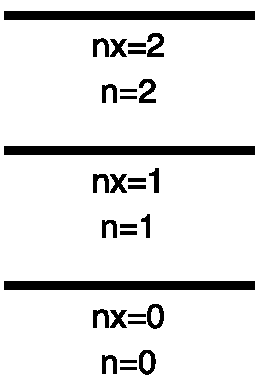
\includegraphics[scale=0.7]{figures/Eigenstates1D}
    \caption{This figure shows the eigenstates for the three lowest energy levels in one dimension. Each line is one eigenstate, and a given eigenstate is on a higher energy level than those below it in the figure. The eigenstates are indexed by $n$, and $nx$ is the quantum number corresponding to the eigenstate. In one dimension we only have one eigenstate per energy level and therefore we always have $nx=n$. However, as seen in Figure \ref{fig: Eigenstates2D} this is not the case for higher dimensions.}
    \label{fig: Eigenstates1D}
\end{figure}

\begin{figure}[!ht]
    \centering
    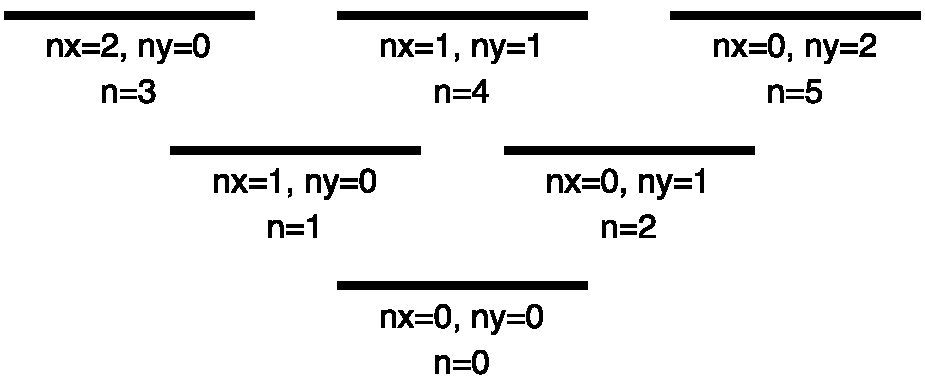
\includegraphics[scale=0.7]{figures/Eigenstates2D}
    \caption{This figure shows the eigenstates for the three lowest energy levels in two dimensions. Each line is one eigenstate and a given eigenstate is on a higher energy level than those below it in the figure. The eigenstates are indexed by $n$. Each eigenstate has two quantum numbers $nx$ and $ny$. Unlike in one dimension (Figure \ref{fig: Eigenstates1D}), when we have two dimensions we can have multiple eigenstates per energy level (e.g. eigenstates $n=1$ and $n=2$).}
    \label{fig: Eigenstates2D}
\end{figure}

%\chapter{Many Particle Theory}

\chapter{Hartree-Fock}

The Hartree-Fock method is well described in \cite{basicMB}, which this chapter is based upon. This method uses an algorithm to find an approximative expression for the ground state of a given Hamiltonian. First we need to define a single particle basis $\left\{\psi_\alpha\right\}$ (e.g. a single particle harmonic oscillator basis), so that 
\begin{equation}
    \hat{h}^{HF}\psi_\alpha = \epsilon_\alpha \psi_\alpha,
\end{equation}
where $\hat{h}^{HF}$ is the Hartree-Fock Hamiltonian
\begin{equation}
    \hat{h}^{HF} = \hat{t} + \hat{u}_{ext} + \hat{u}^{HF}.
\end{equation}
The goal of the Hartree-Fock algorithm is to determine the single particle potential, $\hat{u}^{HF}$, so that we find a local minimum for
\begin{equation}
    \langle \hat{H} \rangle = E^{HF} = \langle \Phi_0 \vert \hat{H} \vert \Phi_0 \rangle,
\end{equation}
where we have a Slater determinant, $\Phi_0$, as the ansatz for the ground state. As with variational Monte Carlo methods, the variational principle ensures that we approach the exact ground state energy, $E_0$, from above, i.e.
\begin{equation}
    E^{HF} \geq E_0.
\end{equation}
We use Hartree-Fock to get coefficients for a self-consistent single particle basis, which we can then use in the VMC calculations instead of the coefficients we got from diagonalizing simple potentials (as described in \ref{sec: Basis Functions}).

\section{Hamiltonian}

If we assume that the interacting part of the Hamiltonian can be approximated by a two-body interaction, we can write the Hamiltonian as
\begin{equation}
    \hat{H} = \hat{H}_0 + \hat{H}_1 = \sum_{i=1}^N \hat{h}_0(x_i) + \sum_{i<j}^N V(r_{ij}),
\end{equation}
where
\begin{equation}
    \hat{H}_0 = \sum_{i=1}^N \hat{h}_0(x_i) = \sum_{i=1}^N \left( \hat{t}(x_i) + \hat{u}_{\textrm{ext}}(x_i) \right)
\end{equation}
is the non-interacting part, and
\begin{equation}
    \hat{H}_1 = \sum_{i<j}^N V(r_{ij})
\end{equation}
is the interacting part. $\hat{t(x_i)}$ represents the kinetic energy of particle $i$, while $\hat{u}_{\textrm{ext}}(x_i)$ represents the one-body part of the potential energy, which can be approximated by a harmonic oscillator potential. $V(r_{ij})$ is the two-body potential between particles $i$ and $j$.

Our Hamiltonian is invariant under permutation of two particles. If we define $\hat{P}$ as an operator which interchanges two particles, due to symmetries in our Hamiltonian, this operator will commute with the total Hamiltonian,
\begin{equation}
    \left[ \hat{H}, \hat{P} \right] = 0.
\end{equation}
This means that the eigenfunction $\Psi_\lambda(x_1,x_2,\dots,x_N)$ of our Hamiltonain is also an eigenfunction of $\hat{P}$, so that
\begin{equation}
    \hat{P}_{ij}\Psi_\lambda(x_1,x_2,\dots,x_i,\dots,x_j,\dots,x_N) = \beta\Psi_\lambda(x_1,x_2,\dots,x_i,\dots,x_j,\dots,x_N),
\end{equation}
where $\beta$ is the eigenvalue of $\hat{P}$ and the $ij$ suffix indicates that we permute particles $i$ and $j$. Since we're looking at fermions, the Pauli principle states that the total wave function has to be antisymmetric, which yields the eigenvaule $\beta = -1$.

We approxiamte the exact eigenfunction with a Slater determinant,
\begin{equation}
    \Phi(x_1,x_2,\dots,x_N,\alpha,\beta,\dots,\nu) = \frac{1}{\sqrt{N!}}
    \left| \begin{array}{ccccc} \psi_\alpha(x_1) & \psi_\alpha(x_2) & \dots & \dots & \psi_\alpha(x_N)\\
                                \psi_\beta(x_1) & \psi_\beta(x_2) & \dots & \dots & \psi_\beta(x_N)\\
                                \dots & \dots & \dots & \dots & \dots\\
                                \dots & \dots & \dots & \dots & \dots\\
                                \psi_\nu(x_1) & \psi_\nu(x_2) & \dots & \dots & \psi_\nu(x_N)

             \end{array} \right|,
      \label{eq:SlaterDet}
\end{equation}
where $x_i$ represent the coordinates and spin values of particle $i$, and $\alpha,\beta,\dots,\nu$ are quantum numbers, while $\psi_\alpha(x_i)$ are eigenfunctions of the one-body Hamiltonian $h_i$, i.e.
\begin{equation}
    \hat{h}_0(x_i) = \hat{t}(x_i) + \hat{u}_\textrm{ext}(x_i),
\end{equation}
and
\begin{equation}
    \hat{h}_0(x_i)\psi_\alpha(x_i) = \epsilon_\alpha\psi_\alpha(x_i).
\end{equation}
The energies $\epsilon_\alpha$ are the unperturbed energies, i.e. the non-interacting single particle energies. With no interaction between particles the total energy would be the sum of these unperturbed energies.

For a given $n\times n$ matrix \textbf{A} the determinant is
\begin{equation}
    \textrm{det}(\mathbf{A}) = \left|\mathbf{A}\right| =
    \left| \begin{array}{ccccc} a_{11} & a_{12} & \dots & \dots & a_{1n}\\
                                a_{21} & a_{22} & \dots & \dots & a_{2n}\\
                                \dots & \dots & \dots & \dots & \dots\\
                                \dots & \dots & \dots & \dots & \dots\\
                                a_{n1} & a_{n2} & \dots & \dots & a_{nn}

             \end{array} \right|,
\end{equation}
which can also be written as
\begin{equation}
    \left|\mathbf{A}\right| = \sum_{i=1}^{n!}(-1)^{p_i} \hat{P}_i a_{11},a_{22},\dots,a_{nn},
\end{equation}
where $\hat{P}_i$ is the permutation operator permuting the column indices, and the sum runs over all $n!$ permutations. The quantity $p_i$ is the number of transpositions of column indices needed to bring a given permutation back to its original ordering.

The Slater determinant from Eq.(\ref{eq:SlaterDet}) is the trial function for the Hartree-Fock method, and we can now rewrite the determinant as
\begin{equation}
    \Phi(x_1,x_2,\dots,x_N,\alpha,\beta,\dots,\nu) = \frac{1}{\sqrt{N!}}\sum_p (-1)^p \hat{P} \psi_\alpha(x_1) \psi_\beta(x_2) \dots \psi_\nu(x_N) = \sqrt{N!} \hat{A} \Phi_H,
\end{equation}
where $\hat{A}$ is the anti-symmetrization operator defined by the summation over all possible permutations of two particles. This operator is given by
\begin{equation}
    \hat{A} = \frac{1}{N!} \sum_p (-1)^p \hat{P},
\end{equation}
with $p$ being the number of permutations. We have also introduced the Hartree-function, defined by the product of all possible single particle functions
\begin{equation}
    \Phi_H(x_1,x_2,\dots,x_N,\alpha,\beta,\dots,\nu) = \psi_\alpha(x_1) \psi_\beta(x_2) \dots \psi_\nu(x_N).
\end{equation}

\section{Expectation Value of the Hamiltonian}

From the variational principle we know that
\begin{equation}
    E_0 \leq E\left[ \Phi \right] = \int \Phi^* \hat{H} \Phi d\tau,
\end{equation}
where $E_0$ is the ground state energy, $d\tau = d\mathbf{r}_1,d\mathbf{r}_2,\dots,d\mathbf{r}_N$, and $\Phi$ is trial function which we assume is normalized, i.e.
\begin{equation}
    \int \Phi^* \Phi d\tau = 1.
\end{equation}

Both the non-interacting part of the Hamiltonian, $\hat{H}_0$, and the interacting part, $\hat{H}_1$, are invariant under all possible permutations of any two particles, and therefore commute with $\hat{A}$
\begin{equation}\label{eq:HA commute}
    \left[ \hat{H}_0, \hat{A} \right] = \left[ \hat{H}_1, \hat{A} \right] = 0.
\end{equation}
In addition, $\hat{A}$ satisfies 
\begin{equation}\label{eq:A2=A}
    \hat{A}^2 = \hat{A},
\end{equation}
since every permutation of the Slater determinant reproduces it. 

\subsection{One-body Hamiltonian}

The expectation value of $\hat{H}_0$ is given by
\begin{equation}
    \int \Phi^* \hat{H}_0 \Phi d\tau = N! \int \Phi_H^* \hat{A} \hat{H}_0 \hat{A} \Phi_H d\tau,
\end{equation}
and using Eq.(\ref{eq:HA commute}) and (\ref{eq:A2=A}), we can reduce it to
\begin{equation}
    \int \Phi^* \hat{H}_0 \Phi d\tau = N! \int \Phi_H^* \hat{H}_0 \hat{A} \Phi_H d\tau.
\end{equation}
Furthermore, we replace the anti-symmetrization operator with its definition, and replace $\hat{H}_0$ with the sum of one-body operators, and obtain
\begin{equation}
    \int \Phi^* \hat{H}_0 \Phi d\tau = \sum_{i=1}^N \sum_p (-1)^p \int \Phi_H^* \hat{h}_0 \hat{P} \Phi_H d\tau.
\end{equation}
If two or more particles are permuted in only one of the Hartree-functions, $\Phi_H$, the integral vanishes since the individual single particle wave functions are orthogonal. We can therefore simplify to
\begin{equation}
    \int \Phi^* \hat{H}_0 \Phi d\tau = \sum_{i=1}^N \int \Phi_H^* \hat{h}_0 \Phi_H d\tau.
\end{equation}
The orthogonality of the single particle wave functions allows us to simplify the integral even more, and we end up with the following expressing for the expectation value of the sum of one-body Hamiltonians
\begin{equation}\label{eq:one-body EV HF}
    \int \Phi^* \hat{H}_0 \Phi d\tau = \sum_{\mu=1}^N \int \psi_\mu^*(\mathbf{r}) \hat{h}_0 \psi_\mu(\mathbf{r}) d\mathbf{r}.
\end{equation}
We introduce the following, more compact, notation for the integral
\begin{equation}
    \langle \mu \vert \hat{h}_0 \vert \mu \rangle = \int \psi_\mu^*(\mathbf{r}) \hat{h}_0 \psi_\mu(\mathbf{r}) d\mathbf{r},
\end{equation}
and rewrite Eq.(\ref{eq:one-body EV HF}) as 
\begin{equation}\label{eq:one-body EV HF 2}
    \int \Phi^* \hat{H}_0 \Phi d\tau = \sum_{\mu=1}^N \langle \mu \vert \hat{h}_0 \vert \mu \rangle
\end{equation}

\subsection{Two-body Hamiltonian}

For the two-body part of the Hamiltonian, we can obtain the expectation value in a similar way as for the one-body part. We start with
\begin{equation}
    \int \Phi^* \hat{H}_1 \Phi d\tau = N! \int \Phi_H^* \hat{A} \hat{H}_1 \hat{A} \Phi_H d\tau,
\end{equation}
and by the same arguments as for the one-body Hamiltonian, we can reduce this to
\begin{equation}
    \int \Phi^* \hat{H}_1 \Phi d\tau = \sum_{i \leq j= 1}^N \sum_p (-1)^p \int \Phi_H^* V(r_{ij}) \hat{P} \Phi_H d\tau.
\end{equation}
Unlike the one-body case, permutations of any two particles doesn't vanish in the two-body case. This is due to the dependence on the inter-particle distance $r_{ij}$. For the two-body case we get
\begin{equation}
    \int \Phi^* \hat{H}_1 \Phi d\tau = \sum_{i \leq j= 1}^N \int \Phi_H^* V(r_{ij}) (1-P_{ij}) \Phi_H d\tau,
\end{equation}
where $P_{ij}$ is the permutation operator for interchanging particle $i$ and particle $j$. As for the one-body case, we assume that the single-particle wave functions are orthogonal, and get
\begin{equation}\label{eq:two-body EV HF}
\begin{split}
    \int \Phi^* \hat{H}_1 \Phi d\tau = \frac{1}{2} \sum_{\mu=1}^N \sum_{\nu=1}^N &\left[ \int \psi_\mu^*(x_i) \psi_\nu^*(x_j) V(r_{ij}) \psi_\mu(x_i) \psi_\nu(x_j) dx_i dx_j\right.\\
    &\left. -\int \psi_\mu^*(x_i) \psi_\nu^*(x_j) V(r_{ij}) \psi_\nu(x_i) \psi_\mu(x_j) dx_i dx_j \right].
\end{split}
\end{equation}
The first term is called the direct term, or the Hartree term, while the second term appears because of the Pauli principle. This term is called the exchange term or the Fock term. Since we now sum over all pairs twice, we need to add a factor $1/2$. The single-particle wave functions $\psi_\alpha(x)$ are defined by the quantum numbers $\alpha$ and $x$ as the overlap
\begin{equation}
    \psi_\alpha(x) = \langle x \vert \alpha \rangle.
\end{equation}
We introduce the following, more compact, notation for the integrals
\begin{equation}
    \langle \mu \nu \vert \hat{v} \vert \mu \nu \rangle = \int \psi_\mu^*(x_i) \psi_\nu^*(x_j) V(r_{ij}) \psi_\mu(x_i) \psi_\nu(x_j) dx_i dx_j,
\end{equation}
and 
\begin{equation}
    \langle \mu \nu \vert \hat{v} \vert \nu \mu \rangle = \int \psi_\mu^*(x_i) \psi_\nu^*(x_j) V(r_{ij}) \psi_\nu(x_i) \psi_\mu(x_j) dx_i dx_j.
\end{equation}
We can define a combination of the direct matrix element and the exchange matrix element which we call the anti-symmetrization matrix element
\begin{equation}
    \langle \mu \nu \vert \hat{v} \vert \mu \nu \rangle_{\textrm{AS}} = \langle \mu \nu \vert \hat{v} \vert \mu \nu \rangle - \langle \mu \nu \vert \hat{v} \vert \nu \mu \rangle,
\end{equation}
which for a general matrix element is 
\begin{equation}
    \langle \mu \nu \vert \hat{v} \vert \sigma \tau \rangle_{\textrm{AS}} = \langle \mu \nu \vert \hat{v} \vert \sigma \tau \rangle - \langle \mu \nu \vert \hat{v} \vert \tau \sigma \rangle.
\end{equation}
This anti-symmetrization element has the symmetry property
\begin{equation}
    \langle \mu \nu \vert \hat{v} \vert \sigma \tau \rangle_{\textrm{AS}} = -\langle \mu \nu \vert \hat{v} \vert \tau \sigma \rangle_{\textrm{AS}} = -\langle \nu \mu \vert \hat{v} \vert \sigma \tau \rangle_{\textrm{AS}},
\end{equation}
and it is hermitian, which implies that 
\begin{equation}
    \langle \mu \nu \vert \hat{v} \vert \sigma \tau \rangle_{\textrm{AS}} = \langle \sigma \tau \vert \hat{v} \vert \mu \nu \rangle_{\textrm{AS}}.
\end{equation}
We can now rewrite Eq.(\ref{eq:two-body EV HF}) as 
\begin{equation}\label{eq:two-body EV HF 2}
    \int \Phi^* \hat{H}_1 \Phi d\tau = \frac{1}{2} \sum_{\mu=1}^N \sum_{\nu=1}^N \langle \mu \nu \vert \hat{v} \vert \mu \nu \rangle_{\textrm{AS}}.
\end{equation}
By combining Eq.(\ref{eq:one-body EV HF 2}) and (\ref{eq:two-body EV HF 2}) we end up with the energy functional 
\begin{equation}
    E\left[ \Phi \right] = \sum_{\mu=1}^N \langle \mu \vert \hat{h}_0 \vert \mu \rangle + \frac{1}{2} \sum_{\mu=1}^N \sum_{\nu=1}^N \langle \mu \nu \vert \hat{v} \vert \mu \nu \rangle_{\textrm{AS}}.
\end{equation}

\section{Polar Coordinates}

If our trial function is a harmonic oscillator function, the integral
\begin{equation}
    \langle \mu \nu \vert \hat{v} \vert \sigma \tau \rangle = \int \psi_\mu^*(x_i) \psi_\nu^*(x_j) V(r_{ij}) \psi_\sigma(x_i) \psi_\tau(x_j) dx_i dx_j,
\end{equation}
can be calculated in analytical form if we use polar coordinates instead of Cartesian coordinates. In two dimensions, using polar coordinates we have
\begin{equation}
    x = r\cos\theta
\end{equation}
\begin{equation}
    y = r\sin\theta
\end{equation}
\begin{equation}
    r = \sqrt{x^2 + y^2},
\end{equation}
and the time independent wave function is composed of a radial part and an angular part
\begin{equation}
    \psi(r, \theta) = R(r)Y(\theta).
\end{equation}
The normalized solution for the angular part in two dimensions is
\begin{equation}
    Y(\theta) = \frac{1}{\sqrt{2\pi}}e^{im\theta}.
\end{equation}
Since the total wave function must satisfy the physical condition
\begin{equation}
    \psi(r, \theta) = \psi(r, \theta + 2\pi),
\end{equation}
the quantum number $m$ is restricted to integral values
\begin{equation}\label{eq:m quantum number}
    m = 0, \pm 1, \pm 2, \dots
\end{equation}
The solution for the radial part is
\begin{equation}
    r_{nm}(r) = \sqrt{\frac{2n!}{(n+|m|)!}} \beta^{\frac{1}{2}(|m|+1)} r^{|m|} e^{-\frac{1}{2} \beta r^2} L_n^{|m|}(\beta r^2),
\end{equation}
where $n$ is the principal quantum number
\begin{equation}
    n = 0, 1, 2, 3, \dots
\end{equation}
and $m$ is the angular momentum quantum number given in Eq.(\ref{eq:m quantum number}). $\beta$ is defined as 
\begin{equation}
    \beta = \frac{m_e \omega}{\hbar},
\end{equation}
where $m_e$ is the particle mass, and $\omega$ is the oscillator frequency. $L_n^{|m|}$ are the associated Laguerre polynomials defined as the solutions to the differential equation
\begin{equation}
    \left( \frac{d^2}{dx^2} - \frac{d}{dx} + \frac{\lambda}{x} - \frac{l(l+1)}{x^2} \right) L(x) = 0,
\end{equation}
where $l$ is an integer $l \geq 0$ and $\lambda$ is a constant. The polynomials for the first few $n$ values are
\begin{equation}
    L_0(x) = 1,
\end{equation}
\begin{equation}
    L_1(x) = 1-x,
\end{equation}
\begin{equation}
    L_2(x) = 2 - 4x + x^2,
\end{equation}
\begin{equation}
    L_3(x) = 6 - 18x + 9x^2 - x^3,
\end{equation}
and
\begin{equation}
    L_4(x) = 24 - 96x + 72x^2 -16x^3 + x^4.
\end{equation}
The Laguerre polynomials fullfill the orthogonality relation 
\begin{equation}
    \int_0^\infty e^{-x} L_n(x)^2 dx = 1,
\end{equation}
and the recursion relation 
\begin{equation}
    (n+1) L_{n+1}(x) = (2n + 1 - x) L_n(x) - n L_{n-1}(x).
\end{equation}
The eigenfunction for a particle moving in a two dimensional harmonic oscillator is then 
\begin{equation}
    \psi(r, \theta) = \sqrt{\frac{n!}{\pi (n + |m|)!}} \beta^{\frac{1}{2}(|m|+1)} r^{|m|} e^{-\frac{1}{2}\beta r^2} L_n^{|m|}(\beta r^2) e^{im\theta},
\end{equation}
with eigenvalue 
\begin{equation}
    E = \hbar \omega (2n + |m| + 1),
\end{equation}
which is the non-interacting energy, similarly to the following expression for Cartesian coordinates 
\begin{equation}
    E = \hbar \omega (n_x + n_y + 1).
\end{equation}


\chapter{Systems}

The systems we are looking at contain electrons confined in a harmonic oscillator like potentials, with the following idealized total Hamiltonian
\begin{align}\label{eq: finalH}
    H=\sum_{i=1}^{N} \left(  -\frac{1}{2} \nabla_i^2 + V_c(\mathbf{r}_i)  \right)+\sum_{i<j}\frac{1}{r_{ij}},
\end{align}
where we have used natural units ($\hbar=c=e=m_e=1$) and all energies are in so-called atomic units a.u. $V_c(\mathbf{r}_i)$ is the external confinement potential at position $\mathbf{r}_i$. Using the above Hamiltonian we will study systems of many electrons $N$ as functions of the oscillator frequency  $\omega$. The unperturbed part of the Hamiltonian is
\begin{align}
    H_0=\sum_{i=1}^{N} \left(  -\frac{1}{2} \nabla_i^2 + V_c(\mathbf{r}_i)  \right),
\end{align}
while the repulsive Coulomb interaction between two electrons is given by
\begin{align}
    H_1=\sum_{i<j}\frac{1}{r_{ij}},
\end{align}
where $r_{ij}=\vert {\bf r}_i-{\bf r}_j\vert$ is the distance between two electrons. The modulus of the positions of the electrons (for a given electron $i$) is defined as $r_i = \sqrt{r_{i_x}^2+r_{i_y}^2}$.



\section{Potentials}

\subsection{Standard Harmonic Oscillator Well}

For the standard harmonic oscillator well, the confinement potential is simply\cite{Griffiths}
\begin{equation}\label{eq: HO Potential}
\begin{split}
    V_c(\mathbf{r}) &= \frac{1}{2}m_e\omega^2 \mathbf{r}^2\\
    &=\frac{1}{2}\omega^2 \mathbf{r}^2,
\end{split}
\end{equation}
where $\mathbf{r}$ is the distance from the center of the well. The potential is zero at the center of the well, and then increases proportionally to $\mathbf{r}^2$ as we move away from the center. Since we use natural units we have $m_e=1$. The strength of the potential is also effected by the constant $\omega$, which is the oscillator frequency. The harmonic oscillator well potential is well studied both analytically and numerically and is therefore good for providing well known benchmarks for our results. The shape of this confinement potential is shown in Figure \ref{fig: HO Potential}.

\begin{figure}[!ht]
    \centering
    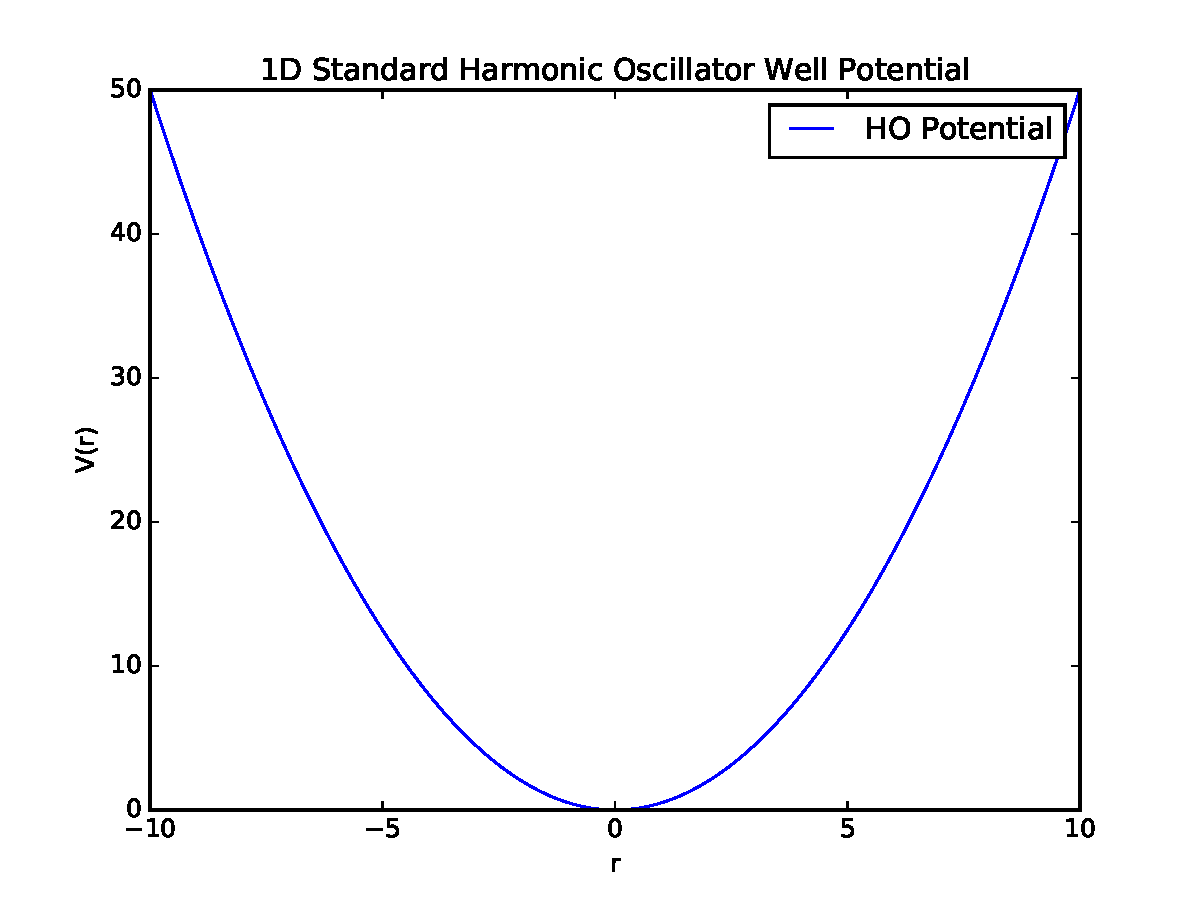
\includegraphics[scale=0.7]{figures/HO_Potential}
    \caption{Standard Harmonic Oscillator Well Potential as described by Eq.(\ref{eq: HO Potential}), with $\omega = 1$.}
    \label{fig: HO Potential}
\end{figure}



\subsection{Double Harmonic Oscillator Well}

When we have a harmonic oscillator potential with multiple minima, the confinement potential is on the general form\cite{master project}
\begin{equation}
    V_c(\mathbf{r}) = \frac{1}{2} m_e \omega^2 \textrm{min}\left[\sum_j^M (\mathbf{r}-\mathbf{L}_j)^2\right],
\end{equation}
where, in two dimensions, we have $\mathbf{r} = (x,y)$, and the multiple $\mathbf{L}_j = (\pm L_x, \pm L_y)$ give the positions of the minima. $M$ is the total number of minima in the potential. When $M=1$ and $\mathbf{L}_1 = (0,0)$ we have the standard harmonic oscillator well, while if $M=2$ and $\mathbf{L}_{1,2} = (\pm L_x, 0)$ we get the double-well potential. We can also write the confinement potential using the absolute values of the coordinates. For a double-well in two dimensions ($\mathbf{L}_{1,2} = (\pm L_x, 0)$) we then get
\begin{equation}\label{eq: DW Potential}
\begin{split}
    V_c(x,y) &= \frac{1}{2} m_e \omega^2[\mathbf{r}^2 - 2L_x|x| - 2L_y|y| + L_x^2 + L_y^2]\\
    &= \frac{1}{2} m_e \omega^2[\mathbf{r}^2 - 2L_x|x| + L_x^2].
\end{split}
\end{equation}
Double-well potentials, and the barrier between the wells, are interesting for quantum computing and information processing. Double-well potentials are investigated as candidates for logic gates in quantum computing\cite{Multiwells}. As explained by Ref.~\cite{Logic Gate}, in regular computing a logic gate is a device implementing a Boolean function. It takes one or more binary inputs and performs a logical operation one them, producing a single binary output. In quantum computing the difference is that the gates should be able to have more varied output, i.e. it should have more output possibilities than only $0$ or $1$. Double-well potentials are also a starting point for understanding periodic multiwell potentials. The double harmonic oscillator potential is parabolic with minima in e.g. $x = \pm L_x$, $y = 0$, and the parabolic wells meet at an absolute value barrier at $x=0$. Figure \ref{fig: DW Potential} shows an example of a double-well potential, where $L_x = 5$ and $\omega = 1$.

\begin{figure}[!ht]
    \centering
    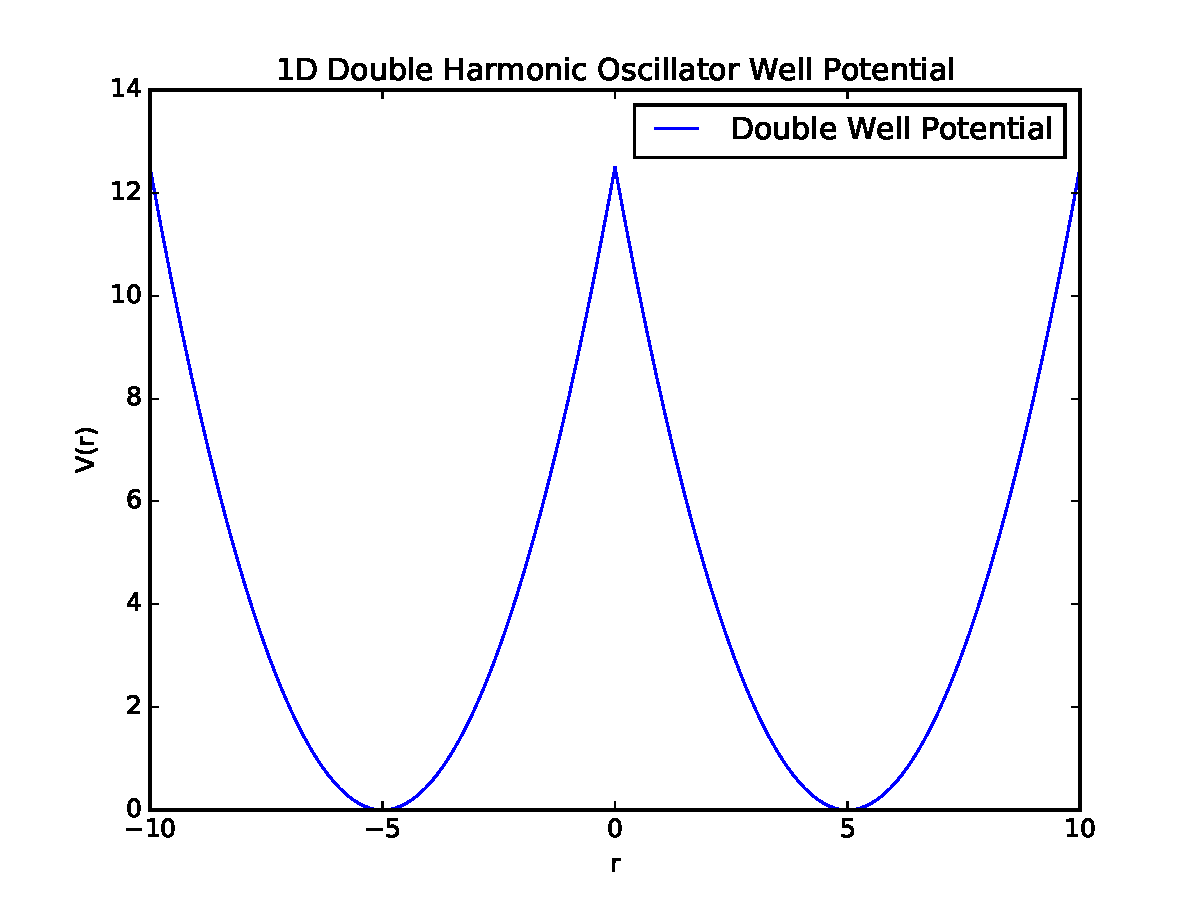
\includegraphics[scale=0.7]{figures/DW_Potential}
    \caption{Double Harmonic Oscillator Well Potential as described by Eq.(\ref{eq: DW Potential}), with $L_x = 5$, $L_y = 0$, and $\omega = 1$.}
    \label{fig: DW Potential}
\end{figure}

\subsection{Finite Square Well}

Another interesting potential to look at is the square well potential, where the potential will have one constant value within the well, and another constant value outside of it. For a finite square well, the potential in one dimension can be written as\cite{Griffiths}
\begin{equation}
    V_c(x) = \begin{cases}
  C_1, & \mbox{if $-L < x < L$} \\
  C_2, & \mbox{otherwise}
\end{cases},
\end{equation}
where $L$ is the distance from the center of the well to the walls, and we have centered the well at $x=0$. For simplicity we set $C_1 = 0$, and rename $C_2$ to $V_0$ which we can then choose as the height of the well. We then have
\begin{equation}\label{eq: FSW Potential}
    V_c(x) = \begin{cases}
  0, & \mbox{if $-L < x < L$} \\
  V_0, & \mbox{otherwise}
\end{cases}.
\end{equation}
This potential has a shape that is somewhat similar to a harmonic oscillator well, and it is also fairly simple since it's either a set constant value or zero, everywhere. Due to it's simplicity this type of potential can more easily be produced in laboratory experiments. Figure \ref{fig: FSW Potential} shows a finite square well potential with $V_0 = 1$ and $L = 3$.

\begin{figure}[!ht]
    \centering
    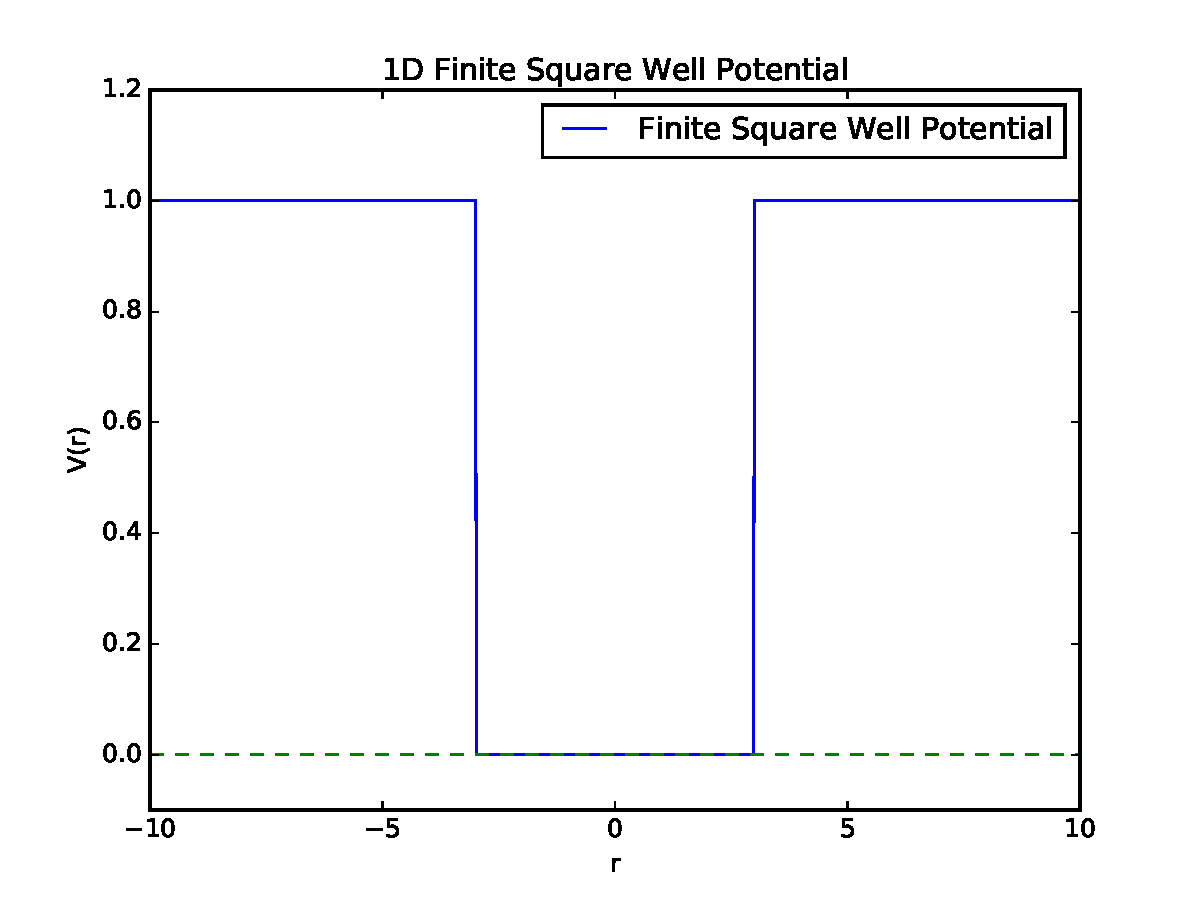
\includegraphics[scale=0.7]{figures/FSW_Potential}
    \caption{Finite Square Well Potential as described by Eq.(\ref{eq: FSW Potential}), with $L = 3$ and $V_0 = 1$.}
    \label{fig: FSW Potential}
\end{figure}


\section{Two-body Quantum Dot}
For two electrons in a two-dimensional harmonic oscillator potential without interaction between the electrons, the energy of each electron is given by
\begin{align}\label{eq: unperturbedEnergy}
    \epsilon_n = \omega(n_x + n_y + 1).
\end{align}
For the ground state we have $n_x=n_y=0$, and since there are two electrons the total (unperturbed) ground state energy is then $\epsilon_0 = 2\omega$. Since electrons are spin-$\frac{1}{2}$ particles they have two possible spin states, which means that both electrons can be in the ground state ($n_x=n_y=0$) as long as they have different spin. One electron will have spin $+\frac{1}{2}$ and the other will have spin $-\frac{1}{2}$, so the total spin of the system will be zero. It makes sense for the ground state to have total spin zero, since the total spin contributes to the energy of the state, and the ground state is the state with lowest energy.

The perturbed trial wave function we will use for the two-body quantum dot has the form 
\begin{align}
    \psi_{T}({\bf r_1},{\bf r_2}) = 
   C\exp{\left(-\alpha\omega(r_1^2+r_2^2)/2\right)}
   \exp{\left(\frac{ar_{12}}{(1+\beta r_{12})}\right)},
\end{align}
where $a=1$ when the electrons have anti-parallel spins and $a=1/3$ when they have parallel spins. For the two-body quantum dot we are interested in the ground state for only two electrons, meaning the electrons will always have anti-parallel spins and $a=1$ in this case. $\alpha$ and $\beta$ are the variational parameters.

\section{Many-body Quantum Dot}
A closed shell system is a system where all used energy levels are filled. This is the case when our number of electrons equal a so-called magic number, i.e. $N=2,6,12,20,\dots$. For a closed shell system with more than two electrons, we use the trial wave function 
\begin{align}
    \psi_{T}({\bf r_1},{\bf r_2},\dots, {\bf r_N}) = 
   Det\left(\phi_{1}({\bf r_1}),\phi_{2}({\bf r_2}),
   \dots,\phi_{N}({\bf r_N})\right)
   \prod_{i<j}^{N}\exp{\left(\frac{a r_{ij}}{(1+\beta r_{ij})}\right)}, 
\end{align}
where $Det$ is a Slater determinant. The single particle wave functions
are harmonic oscillator wave functions with the following form
\begin{align}\label{eq: HO SPWF}
    \phi_{n_x,n_y}(x,y) = A H_{n_x}(\sqrt{\omega}x)H_{n_y}(\sqrt{\omega}y)\exp{(-\omega(x^2+y^2)/2}.
\end{align}
The functions $H_{n_x}(\sqrt{\omega}x)$ are Hermite polynomials \cite{Hermite}, and $A$ is a normalization constant. In this case, two chosen electrons can have either anti-parallel or parallel spins, so the value of $a$ depends on which two electrons we are looking at.

\section{Closed Form Expressions}\label{sec:CF}
We want to find the expectation value of the local energy, and having a closed form expression for this energy is convenient. The local energy is given by 
\begin{align}\label{eq: E_L}
    E_L({\bf R})=\frac{1}{\Psi_T({\bf R})}H\Psi_T({\bf R}).
\end{align}
By finding the local energy using two different methods, one using the closed form expression and the other using a purely numerical approach, we can compare the results of the methods to each other to verify that the program works properly. Using the closed form expression is also computationally faster than the numerical approach, which is convenient when doing large simulations. We can also use closed form expressions for the drift term in importance sampling 
\begin{align}
    F = \frac{2\nabla \Psi_T}{\Psi_T}.    
\end{align}
The necessary closed form expressions for the two-body quantum dot and the many-body quantum dot are calculated in the first appendix, in section \ref{sec:ClosedFormTwo} and section \ref{sec:ClosedFormMany} respectively.

\section{Benchmarks for Verifying the Implementation}
In order to verify that the implementation works correctly we should compare our results with known benchmarks. In the unperturbed case the exact ground state energies are analytically known. We have that the energy for a given electron is given by Eq.(\ref{eq: unperturbedEnergy}). Table \ref{tab: unperturbedEnergies} contains the total energy of unperturbed closed shell systems up to $N=20$ electrons.
\begin{table}[!ht]
  \centering
  \begin{tabular}{ | c | c | }
    \hline
     $N$ & $E$ \\*
    \hline
     $2$ & $2\omega$ \\*
    \hline
     $6$ & $10\omega$ \\*
    \hline
    $12$ & $28\omega$ \\*
    \hline
    $20$ & $60\omega$ \\*
    \hline
  \end{tabular}
  \caption{Benchmarks of the energy $E$ for unperturbed closed shell systems in two dimensions with $N$ electrons.}
  \label{tab: unperturbedEnergies}
\end{table}

For the perturbed case we use the benchmarks given in table \ref{tab: perturbedEnergies} provided by Ref.~\cite{QDotBenchmarks}. From Ref.~\cite{Taut} we also have an analytical result for the ground state energy, $E=3$, for the two-body case with $\omega=1$.
\begin{table}[!ht]
  \centering
  \begin{tabular}{ | c | c | }
    \hline
     $N$ & $E$ \\*
    \hline
     $2$ & $3.000$ \\*
    \hline
     $6$ & $20.1597$ \\*
    \hline
    $12$ & $65.700$ \\*
    \hline
    $20$ & $155.868$ \\*
    \hline
  \end{tabular}
  \caption{Benchmarks of the energy $E$ for perturbed closed shell systems in two dimensions with $N$ electrons and $\omega=1$.}
  \label{tab: perturbedEnergies}
\end{table}


\end{document}